$\arg(z) =
\begin{cases} 
    0                                                & \text{if } \Re(z) \geq 0 \land \Im(z) = 0 \quad | \quad \text{CASE 1}\\
    \arctan\left(\frac{\Im(z)}{\Re(z)}\right)        & \text{if } \Re(z) > 0 \land \Im(z) > 0 \quad | \quad \text{CASE 2}\\
    \frac{\pi}{2}                                    & \text{if } \Re(z) = 0 \land \Im(z) > 0 \quad | \quad \text{CASE 3}\\
    \arctan\left(\frac{\Im(z)}{\Re(z)}\right) + \pi  & \text{if } \Re(z) < 0 \qquad \qquad \qquad \quad| \quad \text{CASE 4}\\
    \pi                                              & \text{if } \Re(z) < 0 \land \Im(z) = 0 \quad | \quad \text{CASE 5}\\
    \frac{3\pi}{2}                                   & \text{if } \Re(z) = 0 \land \Im(z) < 0 \quad | \quad \text{CASE 6}\\
    \arctan\left(\frac{\Im(z)}{\Re(z)}\right) + 2\pi & \text{if } \Re(z) > 0 \land \Im(z) < 0 \quad | \quad \text{CASE 7}
\end{cases}$

\begin{center}
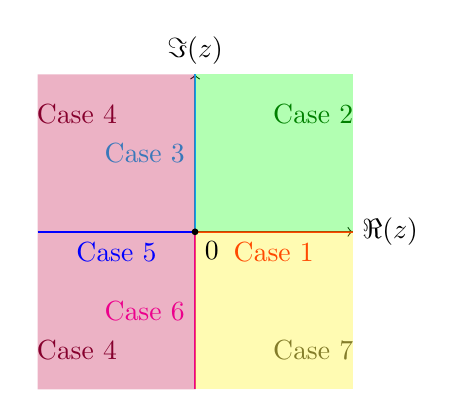
\begin{tikzpicture}[scale=1]
    % Axes
    \draw[->] (-2,0) -- (2,0) node[right] {$\Re(z)$};
    \draw[->] (0,-2) -- (0,2) node[above] {$\Im(z)$};
    
    % Regions
    % Case 1: Re(z) >= 0 and Im(z) = 0 (positive real axis)
    \draw[thick, red] (0,0) -- (2,0) node[midway, below] {Case 1};
    
    % Case 2: Re(z) > 0 and Im(z) > 0 (upper-right quadrant)
    \fill[green, opacity=0.3] (0,0) -- (0,2) -- (2,2) -- (2,0) -- cycle;
    \node[green!50!black] at (1.5,1.5) {Case 2};
    
    %  Case 3: Re(z) = 0 and Im(z) > 0 (positive imaginary axis)
    \draw[thick, cyan] (0,0) -- (0,2) node[midway, left] {Case 3};
    
    \fill[purple, opacity=0.3] (0,0) -- (0,2) -- (-2,2) -- (-2,-2) -- (0,-2) -- cycle;
    % Case 4: Re(z) < 0 and Im(z) > 0 (upper-left quadrant)
    \node[purple!70!black] at (-1.5,1.5) {Case 4};
    % Case 4: Re(z) < 0 and Im(z) < 0 (lower-left quadrant)
    \node[purple!70!black] at (-1.5,-1.5) {Case 4};
    
    % Case 5: Re(z) < 0 and Im(z) = 0 (negative real axis)
    \draw[thick, blue] (0,0) -- (-2,0) node[midway, below] {Case 5};
    
    % Case 6: Re(z) = 0 and Im(z) < 0 (negativ imaginary axis)
    \draw[thick, magenta] (0,0) -- (0,-2) node[midway, left] {Case 6};
    
    % Case 7: Re(z) > 0 and Im(z) < 0 (lower-right quadrant)
    \node[yellow!20!black] at (1.5,-1.5) {Case 7};
    \fill[yellow, opacity=0.3] (0,0) -- (0,-2) -- (2,-2) -- (2,0) -- cycle;
    
    % Origin
    \filldraw[black] (0,0) circle (1pt) node[below right] {$0$};
\end{tikzpicture}
\end{center}
\label{fig:Arg-cases}
